\chapter{Computational Models for Disordered nanowire networks and Their Application}
The aim of this chapter is to introduce the computational framework to numerically calculate the sheet resistance of a nanowire network where inner wire resistance is both included and excluded is introduced. A method to digitise Scanning-Electron-Microscope images of nanowire networks is presented allowing for simulations on a near identical network connectivity with physical networks whose resistance has been experimentally measures. The matching network geometry in computer simulations and inclusion of inner-wire resistance provide an estimate for the inter-wire junction resistance and is shown to be close to resistances measured experimentally. A method to determine the ultimate conductivity of a nanowire network, i.e. where network resistance is due to inner-wire resistance only, is presented and applied to several experimental samples. Aspects of theis work have been published in ...
\newpage
\section{Motivation}
The conductance of a nanowire network (NWN) depends on a multitude of parameters; length and diameter distributions of nanowires\cite{hecht2006,bergin2012,sorel2012,hicks2009,pike1974}, inter-wire junction resistances\cite{mutiso2013}, inner-wire resistance of wire segments{\cite{zezelj2012}, wire density\cite{balberg1983}}, and electrode shape \cite{fairfield2014}. All of these parameters combine to give a unique connectivity profile for each NWN which determines its conductance. One way of numerically solving this percolative transport problem\cite{kirkpatrick1973} is to map the NWN onto a node-voltage graphical representation where each nanowire is a Node in the graph and is connected to its nearest neighbours by a resistor corresponding to the junction resistance between these wires. With the graphical representation one can simply apply Ohm's and Kirchoff's current laws to the graph and calculate the conductance of the network\cite{graph_book}. An implicit assumption is being made in this approach, the junction resistance is much higher than the inner-wire resistance of the NWNs themselves and so dominate the electrical properties of the network. This approach shall be referred to as the Junction Dominated Assumption (JDA) henceforth and importantly one should note it does not contain the effects of inner-wire resistances.
%With such a large parameter space determining a relationship between the conductance of a NWN and the underlying parameters is difficult, requiring fitting of empirical functions to the results of large scale Monte Carlo simulations.

Previously the JDA approach has been used successfully to model networks made of Carbon Nanotubes \cite{nirmalraj2009,hecht2006} where the resistivity of the carbon nanotubes are negligible compared to the resistance of a nanotube junction.  However metallic nanowire junctions have been shown to have a relatively low resistance\cite{bellew2015} and as a result the resistance of the nanowires themselves is comparable to the junction resistance. In this scenario the JDA will not capture the electrical properties of the NWN, previous Monte Carlo simulations of homogeneous conductive networks show that the electrical properties are dependent on the ratio $R_{in}/R_{j}$\cite{li2009,hicks2009,zezelj2012}. Demand for low sheet-resistance, high optical transparency NWNs for use in transparent conductive devices such as solar-cells, capacitive touch screens and others\cite{madaria2010, sakunta2009,sukanta2011} has lead to the use of annealing techniques to minimise the inter-nanowire junction resistance. Decrasing the junction resistance causes them to become comparable with inner-wire resistances and so their effect must be included in models of the network. In this Chapter we introduce such a model, the Multi-Nodal Representation (MNR), and show how both MNR and JDA models depend on the underlying parameters mentioned at the start of the Chapter.

A fundemental issue with nanowire network simulations is the inherent spatial randomness of wire positions and their impact on network connectivity. Experimental measurements can only be related to the avereage results of Monte Carlo simulations with the same underlying parameters in order to obtain meaninful results\cite{mutiso2013}. This approach however fails to give a complete understanding of the electrical properties of the individual NWN, merely an understanding of how it compares to the average. To directly compare computational simulation with experimental measurements we developed a method to digitally capture the positions and orientations of nanowires from Scanning-Electron-Microscope images of NWNs which allows simulations to be performed on networks with a geometry matching that of the experimental sample. This approach allows calculated sheet resistances to be compared directly with experimentally measured sheet resistances, removing geometrical randomness from the comparison. The goal of this Chapter is to compare MNR and JDA simulations using both configurational averaging and digitised networks with experimental samples to understand the effect of inner-wire resistance on the network.

The layout of this Chapter is as follows. In Section \ref{sec:Graphical Representations of NWNs} The JDA and MNR models are presented and the computational simulations are outlined. In Sections \ref{Sec: Resistive properties} \& \ref{Sec: geometric_properties} MNR and JDA are applied to simulations of NWNs and the effect of the various parameters of the NWNs are explored. The dependence of MNR on the inner-wire resistances and the effect of the junction resistance in both models are presented in Section \ref{Sec: Resistive properties}. The dependence of wire densities and wire lengths are determined through spatial configurational averaged simulations in Section \ref{Sec: geometric properties}. In Section \ref{sec:image_proc} images of experimental NWNs are processed and the JDA and MNR are applied to the digitised network. The digitised network can be used to approximate the junction resistance of the samples and these approximations were compared with a distribution of junction resistances that were experimentally measured by Bellew et al\cite{bellew2015}. The Ultimate Conductivity of a NWN, that which is obtained when junctions are annealed to perfect conductors, is calculated for each of the experimental samples. A dimensionless parameter that illustrates the potential for network conductance improvement is introduced and its dependence on several network parameters are presented. There is a short Chapter summary in Section \ref{sec:Conclusion}.

\section{Graphical Representations of Nanowire Networks}
\label{sec:Graphical Representations of NWNs}

To calculate the global resistive properties of the NWN it must be mapped into a node voltage problem, essentially capturing the connectivity information of a NWN in a mathematical graph so that Kirchoff's matrix equations introduced in Chapter 2 can be used. In the Junction Dominated Asspumption (JDA) mapping each wire is represented by a circuit node at a common voltage connected to other wires by a certain number of junction resistors determined by its connectivity within the network. A NWN with $N_w$ wires will result in a resistive graph with $N_w$ nodes. An off-diagonal element of the Kirchoff matrix ($K^{jda}_{ij}$) is the conductance of the wire junction between wires $i$ and $j$ (the conductance is 0 if there is no junction between the wires). Figure \ref{fig: mnr_jda_sketch}(a) is a sketch of a simple NWN (top) with its graphical representation (bottom) where there are three nodes, one for each nanowire, and two inter-wire junctions represented by the dotted line with a resistance $R_j$. Note that there is no junction between wires $W_1$ and $W_2$ thus there is no resistor depicited in the graphical representaion. The locations of the nanowires are irrelevant in the JDA, it is only the connectivity profile of the network that determines the electrical properties. As this mapping only acts on the inter-wire connectivity the electrical properties of the inner-wire segments are entirely omitted from this model.

\fig{1.0}
{Images/Chapter3/mnr_jda_sketch_lowQ.png}
{\textbf{Schematic:} JDA Sketch}
{ a) A sketch of a simple NWN with 3 wires labeled $W_i$ $i = 1,2,3$ and two inter-wire junctions, one between wires $W_1$ and $W_2$ and another between wires $W_1$ and $W_3$. Underneath the sketch is a graphical representation of the NWN, there are three nodes corresponding to the three wires and two inter-wire junction resistors represented by black resistors and labelled $R_j$. b) An expanded view sketch of a simple NWN with 3 wires with two inter-wire junctions. The 4 connection nodes, two for each inter-wire junction, are shwon as the red dots labelled $C_i, ~ i=1,2,3,4$. Underneath the sketch is an MNR graphical representation of the NWN. Connection nodes associated with the same junction are connected by a junction resistor $R_j$ and shown in black. The connection nodes that are adjacent on wire 3, $C_2$ and $C_4$ are connected by an inner-wire segment resistor $R_{in}$ illustrated by the yellow resistor. Note: Image quality to be updated}
{fig: mnr_jda_sketch}


% MNR
While the JDA is suitable for materials with a large junction resistance the inner-wire resistance cannot be omitted for materials where it is comparable with that of the junctions. In order to include the inner wire resistances a new voltage-node mapping is needed. Consider a wire that has $b$ intersections with other wires thus partitioning it into $b+1$ wire sections each with a classical resistance given by 
\begin{equation}
R_i = \frac{\rho \ell_i}{A}
\end{equation}
Where $\rho$ is the wire's resistivity, $\ell_i$ is the length of wire section $i$ and A is the cross sectional area of the wire. Note that two of the sections, at either end of the nanowire, play no part in the electrical properties of the network as they in a sense `dead-ends' for current flow\cite{ocallaco2016}. The interwire connection points, which partition the wire segments, are a natural choice for the nodes in the new node-voltage mapping which we shall call Multi-Nodal Representation (MNR) henceforth. For each inter-wire junction there are two connection nodes, one on each wire, and are connected by a junction resistor. Adjacent connection nodes on the same nanowire are joined with an inner-wire resistor. A sketch of a simple NWN and the corresponding MNR graphical representation is presented in Figure \ref{fig: mnr_jda_sketch}(b). The total number of nodes in this scheme is $2 N_j=4$ where $N_j=2$ is the total number of junctions in the network. Unlike the JDA model, the spatial configuration of the wires and their intersections in the network is required in the MNR model as the distances between adjacent connection nodes is needed for the calculation of inner-wire resistances. If two nodes share the same (x,y) coordinates then they are associated with the same inter-wire junction and are on different wires. 

Consider a NWN with $N_w$ wires and $N_j$ junctions. The number of current carrying wire segments $N_{cc}$ in the network are the number of wire segments $N_s$ minus two 'dead-ends' per wire.
\begin{equation}
N_{cc} = N_s - 2 N_2
\end{equation}
For every intersection on a wire, an additional wire segment occurs on it. Following this logic the number of wire segments is $N_w$ initially and for every junction in the NWN there are two wire segments created, an additional segment on each wire. Thus the total number of wire segments are 
\begin{equation}
N_s = 2N_j + N_w
\end{equation}
The number of current carrying wire segments is thus 
\begin{equation}
N_{cc} = N_s - 2 N_w = 2 N_j - N_w
\end{equation}
In Chapter 2 the relationship between the junction density was related to the wire density in a network by $n_j = a L^2 n_w^2 $ meaning that the total number of junctions is $N_j = a L^2 N_w^2 / B$ where $L$ is the length of each wire, $B$ is the total area of the NWN and $a$ is a constant $\approx 0.318$. The corresponding Kirchoff matrix for the JDA model has $N_w^2$ elements in it with $N_j$ unique values. The MNR model Kirchoff matrix on the other hand has $4 N_j^2$ elements containing $ N_j + N_{cc} = 2 N_j - N_w $ unique elements. The MNR model requires and additional $N_j - N_w$ elements then needed for the JDA to solve the electrical properties of a NWN. This comparison between the information needed to solve the electrical properties of a NWN highlight one of the key problems of the MNR model, the amount of information stored by the model is much higher than the JDA model and so is more limited by computational memory. Furthermore the computational power to solve a set of $2 N_j$ linear equations in the MNR model is an order of magnitude higher than needed for the JDA model, i.e. $O(N_w^2)$ for the MNR versus $O(N_w)$ for the JDA.

In both JDA and MNR the computational simulations are performed as follows. A number of nanowires with a given length, random positions, and random orientations are simulated. Where two wires intersect with one-another an inter-wire junction occurs, the positions and associated wires of each intersection are then determined. The MNR and/or JDA mapping can be applied to the NWN with the connectivity profile and the wire positions. The Kirchoff matrix for both can be formulated and numerically solved to calculate the sheet resistance of the network. The same network can be recreated a number of times by simply choosing the same random number generator seed used to generate the positions and orientations of wires in simulations allowing the impact of particular network parameters to be assessed. The two models are an excellent tool to determine the effect of all of the underlying properties on the resulting sheet resistance of the NWN. 

The properties of the NWN can be grouped into two main categories, the Geometrical parameters and the Resistive parameters. The Geometrical parameters are those that effect the actual connectivity of the NWN; the wire density ($n_w$) and wire length ($L$). Wire diameters are not used to determine the intersection of two nanowires and so is not included as a Geometrical paramter. A change in one of these parameters totally changes the connectivity profile of the NWN and two networks with the same wire lengths and densities can have vastly different sheet resistances due to stochastic fluctuations. To combat this Monte Carlo simulations are performed whereby a large number of NWNs are generated for each combination of wire density and wire lengths and so the effect of each parameter can be determined. The Resistive parameters do not alter the connectivity profile of the NWN but change the magnitude of the resistors in the network. These are the junction resistance ($R_j$), the wire resistivity ($\rho$) and the wire diameter $D$. The effect of these parameters are best illustrated by fixing a NWN connectivity profile and calculating the change in sheet resistance associated with changes to these parameters. The effect of these two categories of parameters will be explored in the proceeding sections. 
%Where possible the properties of the nanowires were kept to those typical of Ag-PVP core shell nanowires that were used extensively in the physical experiments performed by colleagues. 
%\todo{add krichoff matrices?}
%================= resistive properties =================================
\section{Impact of Resistive Parameters on nanowire network Resistance}
\label{Sec: Resistive properties}
The resistive properties of nanowires do not alter the connectivity of the NWN but they do however change the resistor values in the connectivity profile. Both JDA and MNR were applied to the same network geometry in order to keep the connectivity profile the same and allow for a direct comparison between models. Figure \ref{fig: plotNW} is a visualisation of the simulated network of size  $20 \mu m \times 20 \mu m$, wire lengths 7 $\mu m$, and wire density 0.4 NW/$\mu m^{-2}$. The wire density and wire lengths were chosen such that the network was well away from the critical density for wires of this length ($\approx 0.11$), thus ensuring an electrical connection between the two electrodes. This network will be the benchmark geometry used to identify the dependence of $R_s$ on $\rho$, $A$ and $R_j$ in this section.

\fig{0.75}
{Images/Chapter3/network.pdf}
{\textbf{Schematic:} nanowire network}
{Plot of a simulated network. Wires are 7 $\mu m$ in length and there is a wire density of 0.4 $\mu m^{-2}$ which is well above the critical density for this wire length. The network has dimensions $20 \mu m \times 20 \mu m$ and the electrodes are represented by the thick red lines vertical lines either side of the network.}
{fig: plotNW}

The common resistive parameter between MNR and JDA is the junction resistance ($R_j$). In this comparison between the models every junction resistance was assigned the same value $R_j$. The resistivity and wire diameters were fixed in the MNR to values typical of Ag/PVP core-shell nanowires, $\rho = 22.6 n \Omega m$ and $D = 50 nm$ \cite{rocha2015}. Figure \ref{fig: junction_res} shows the effect of increasing $R_j$ on the calculated sheet resistance for both the MNR and JDA models. A striking feature of Figure \ref{fig: junction_res} is that the sheet resistance of the MNR and JDA depends linearly on the junction resistance. Furthermore the slope of the linear relationship is the same in both models, 
\begin{align}
R_s^{JDA} &= a R_j  \label{eq: Rs_jda}\\
R_s^{MNR} &= a R_j + R_0 \label{eq: Rs_mnr}
\end{align}
($a \approx 0.37$ and $R_0 \approx 21 \Omega$ in this case). Intuitively the JDA functional form behaves as desired, one expects a sheet resistance of 0 if every junction in the network has 0 resistance. Similarly the MNR functional behaves as expected, as the junction resistance is brought to 0 the sheet resistance tends to the inner-wire resistance of the network $R_0$. The inclusion of the inner-wire resistance drastically increases the sheet resistance for a given junction resistance for this NWN. For example, in the MNR model the $R_s = R_0 = 21\Omega$ for $R_j = 0$. In order to achieve this sheet resistance in the JDA the junction resistance required is $R_j = 21/a \approx 60 \Omega$. This difference between the required $R_j$ in both models can cause their overestimation when comparing simulations and experiments and is discussed further a later section.

The value of the slope for both models ($a$) allows for an understanding of the nature of current flow through the NWN. A NWN is a mass of parallel paths between the two electrodes, all of varying length. A simple interpretation of current flow through the NWN is that there are $P$ parrallel paths of $S$ junction resistors in series. $S$ and $P$ are characteristic parameters unique to each network. The sheet resistance of such a network in the JDA model is 
\begin{equation}
R_s = \frac{S R_j}{P} 
\end{equation}
Comparing this to equation \ref{eq: Rs_jda} shows that $a = \frac{S}{P}$. Thus for $a<1$ we can argue that the current flow through the NWN is through many parallel paths $P$, more paths than the number of junctions connected in series $S$. If $a>1$ then the current flows through few paths between electrodes. One expects that $a$ depends on the connectivity profile, where highly connected NWNs will have a much lower slope than sparse networks.

\fig{1}
{Images/Chapter3/Junction_resistance.pdf}
{\textbf{Plot:} Junction Resistance}
{The effect of the resistance of each junction in the network on the sheet resistance of the network shown in Fig. \ref{fig: plotNW}. The sheet resistance $R_s$ depends linearly on the junction resistance for both the MNR and JDA models. In fact the slope of both linear functions ($a$) is the approximately the same for both functions at $a \approx 0.37$. The effect of the inner-wire resistance in the MNR manifests as the addition of a constant $R_0$ and corresponds to $R_s^{MNR}$ with $R_j = 0$.}
{fig: junction_res}

A symmetry argument of sorts can be made to explain the linear relationship between $R_s$ and $R_j$ in the JDA whereby if the only difference between two networks is a constant shift of every resistors value then the resistance between any nodes in the network should shift by the same amount. A mathematical proof of this can also be made by making use of the Kirchoff Matrix formalism defined in Chapter 2. If every resistor in the NWN has the same value $R$ then the Kirchoff matrix is 
\begin{equation}
\hat{K} = \frac{1}{R} \hat{\mathcal{L}} = \Gamma \hat{\mathcal{L}}
\end{equation}
recalling that $\hat{\mathcal{L}}$ is the Laplacian matrix defined in Chapter 2. The Kirchoff matrix, along with the current vector which denotes the input and output current to the network $\vec{I}$, is used to solve the potential at each node in the network. Consider the case where $R = 1$
\begin{equation}
\hat{\mathcal{L}} \vec{V}^\mathcal{L} = \vec{I} 
\label{eq: temp}
\end{equation}
where $\vec{V}^\mathcal{L}$ is the solution to this equation. The resistance between the input node (label m) and the output current node (label n) is
\begin{equation}
R^L_{mn} = \frac{| \vec{V}^\mathcal{L}_m - \vec{V}^\mathcal{L}_n|}{i_0}
\end{equation}
where $i_0$ is the current flowing between the nodes. Now consider the case where $R \neq 1$ and the current vector is the same as before. We now have
\begin{equation}
\hat{K}\vec{V} = \frac{1}{R}\hat{\mathcal{L}}\vec{V}^k = \vec{I}
\end{equation}
Using equation \ref{eq: temp} we can equate $ \frac{1}{R}\hat{\mathcal{L}}\vec{V}^k = \hat{\mathcal{L}}\vec{V}^\mathcal{L}$ and so the Voltage vectors are related by
\begin{equation}
\vec{V}^k = R \vec{V}^\mathcal{L}
\end{equation}
The resistance between the two nodes m and n are now
\begin{equation}
R^K_{mn} = R \frac{| \vec{V}^\mathcal{L}_m - \vec{V}^\mathcal{L}_n|}{i_0}
\end{equation}
proving that the resistance between two nodes in a network of identical resistors depends linearly on their resistance. This method cannot be easily applied to the MNR model as the Kirchoff matrix also contains inner-wire resistances which are variable.

The wire resistivity and cross sectional area are unique to the MNR and so a comparison with JDA cannot be performed for these parameters. Their effect on $R_s$ was determined by applying the MNR model to the NWN pictured in Figure \ref{fig: plotNW} with $R_j =11 \Omega$. Figure \ref{fig: mnr_resistivity_diameter} a) shows the effect of changing the resistivity on the sheet resistance. $R_s$ clearly increases in a linear fashion with respect to increasing resistivity which can be attributed to the linear dependence of the resistance of wire segments on the resistivity thus shifting $R_0$ in the linear formula for $R_s$ given in Equation \ref{eq: Rs_mnr}. Figure \ref{fig: mnr_resistivity_diameter} b) Shows the effect of increasing wire diameter ($D$) on the sheet resistance of a network. The sheet resistance decreases as a power law relationship, $R_s = c  D^{-2} + aR_j$, which is as expected as the inner-wire resistance depends on the wire diameter in this way. This power-law relationship is clearly evident in the inset plot which is the same data in logscale alongside a curve defined by $c  D^{-2} + aR_j$ which was included as a guide to the eye. The curve has been offset to the experimental data for ease of viewing. If one were to consider a NWN with perfect junctions ($R_j = 0$) then a scaling argument similar to that used to describe the linear dependence of $R_s$ on $R_j$ can be used to describe the relationships $R_0 \propto \rho D^{-2}$.

Note that a non-zero junction resistance was used in simulations and so the sheet resistance tends to a non-zero value for vanishing resistivity and infinite wire diameter, $R_s \rightarrow a R_j$ as $R_0 \rightarrow 0$. This asymptotic sheet resistance is represented by the dashed horizontal line in both plots of Figure \ref{fig: mnr_resistivity_diameter}. As the sheet resistance does not tend to a zero value the curves in the logplot in the inset of Figure \ref{fig: mnr_resistivity_diameter}(b) gradually become more horizontal for increasing wire diameter.

\fig{1.}
{Images/Chapter3/resistivity_wireDiameter.pdf}
{\textbf{Plot:} Resistivity Parameters}
{a) The dependence of $R_s$ on the resistivity of the nanowires, specific to the network geometry shown in Figure \ref{fig: plotNW}. $R_s$ depends linearly on the resistivity of the nanowires, the same dependence that the inner-wire dependence has on the resistivity. b) The dependence of $R_s$ on the diameter of the nanowires $(D)$, again this relationship is as expected with a $D^{-2}$ dependence similar to the inner-wire resistance dependence on $D$. In the inset the same data is replot in Log-scale in blue. The black dashed line is a guide-to-the-eye curve determined by the equation $c D^{-2} + a R_j$ where c is a constant, note that the equation has been off-set from the data for ease of viewing. Recall $R_s = a R_j + R_0$ and so the sheet resistance tends to a non-zero value determined by the junction resistance for vanishing inner-wire resistance. The horizontal dashed line in both plots represents the sheet resistance with no inner-wire resistance $R_s = aR_j \approx 4.07 \Omega$.}
{fig: mnr_resistivity_diameter}

%------------------------------ scaling properties? --------------------------
\section{Impact of Geometric Paramters on nanowire network Resistance}
\label{Sec: geometric_properties}
The geometric parameters that are common to both the JDA and MNR models are the wire density and wire lengths. Altering either of these parameters results in a fundamental change in the in the connectivity profile. This change is best illustrated by the expression for the junction density derived in Chapter 2, $n_j = a L^2 n_w^2$ as it is the junctions that determine the connectivity profile. Recall from the definitions of the JDA and MNR they are a source of resistance and determine the graphical representations of the NWN. As discussed in Chapter 2, Percolation theory can be used to determine quantities such as the critical wire density, below which a conductive path does not form between electrodes. This is described using the equation 
\begin{equation}
(n_w)_c = 5.63726 L^{-2}
\label{eq: critical_wire_density}
\end{equation}
This equation can be furthered to calculate a critical wire length for a given wire density by simply setting $L \rightarrow L_c$ and $(n_w)_c \rightarrow n_w$ in Equation \ref{eq: critical_wire_density}. 
According to percolation theory, the sheet conductance $\Gamma_s$ of a random stick network scales as a power law with the stick density as a power law
\begin{equation}
\Gamma_s \propto (n_w - (n_w)_c)^{-\beta}
\label{eq: percolation_scaling}
\end{equation}
Where $(n_w)_c$ is the critical wire density discussed above. This scaling law has been well documented in simulations\cite{pike1974,li2009,zezelj2012} and has been used to understand the scaling of Carbon Nanotube networks and metallic nanowire networks\cite{hu2004,bergin2012}

The effect of wire density on the average $R_s$ calculated in JDA (blue) and MNR (red) for a number of NWNs is displayed in Figure \ref{fig: wireDensity}(a). Other parameters were set to values obtained for Ag PVP core shell nanowires\cite{rocha2015} that were used in the previous section; $L = 6.7 \mu m$, $R_j = 11 \Omega$, $D = 50 n m$, and $\rho = 22.6n\Omega m$. The wire lengths are not too long as to cause finite sized effects, i.e. where the distance between electrodes could be bridged by a single wire. 20 simulations were performed for a given wire density in order to obtain an accurate calculation of $R_s$ and the associated confidence interval. 

From Figure  \ref{fig: wireDensity}(a) the MNR model has a higher sheet resistance for the JDA model at same densities. This is unsurprising due to the inclusion of inner-wire resistance for the MNR model and the junction resistances being the same in both models. There is large uncertainty for the average $R_s$ for simulations at lower densities due to being close to the critical density of $(n_w)_c = 0.11$NW$/\mu m$ according to Equation \ref{eq: critical_wire_density}. A sparse network is susceptible to the stochastic effects of the network and the large uncertainty in the sheet resistance results. The general decreasing trend of the sheet resistance with increasing nanowire is understood as the network develops more pathways between the electrodes. 

\fig{1.}
{Images/Chapter3/wire_dens_final.pdf}
{\textbf{Plot:} Wire density}
{(a) The effect of changing wire density $n_w$ on sheet resistance $R_s$ for networks of size $20\mu m \times 20 \mu m$ and wires of length $7 \mu m$. The wire resistivity, cross sectional area and junction resistance are those measured typical for Ag PVP core shell nanowires. 20 random networks were simulated for each wire density in both MNR and JDA and the average sheet resistance and 95\% confidence interval for each wire density was calculated and plot. (b) Sheet resistance versus the parameter ($n_w - (n_w)_c$) for comparison with Equation \ref{eq: percolation_scaling}. Here the two scaling regimes between $R_s$ and $n_w$ is evident for both models. Power-laws were fit to both models and are shown as dotted lines. For the MNR model the scaling exponent according to regression analysis is $\beta_{MNR} \approx 1.28$ and the fitted curve is shown as the black dashed line. The JDA line has an exponent $\beta_{JDA} \approx 1.44$ and is shown as the green dashed line.}
{fig: wireDensity}

Figure \ref{fig: wireDensity}(b) recasts the data from Figure (a) in a logscale plot and altering the horizontal axis to $(n_w - (n_w)_c)$ for comparison with the power-law scaling of percolation theory outlined in Equation \ref{eq: percolation_scaling}. Both MNR and JDA have a power law response to the increase in wire density that is easily identifiable in this plot. The Power-law $R_s \propto (n_w - (n_w)_c)^{-\beta}$ were fit to both curves and the two models were found to have differing exponents, $\beta_{MNR}\approx -1.28$ (black dashed line) and $\beta_{JDA}\approx -1.44$ (green dashed line). These exponents are in line with those seen in Monte Carlo simulations that have been reported in the literature. Li and Zhang showed that for wire densities in the range $0.3 \leq (n_w/(n_w)_c - 1) \leq 1$ and wires of unit length the scaling exponent depends on the ratio of junction resistance to inner-wire resistance ($R_i$). By fitting the Error function to Monte Carlo simulations they found the relationship between the scaling exponent and $x = \log_{10}(R_j/R_i)$ was 
\begin{equation}
\beta = \beta_0 + C~ erf(x)
\end{equation}
where $t_0 = 1.314 \pm 0.002$ and $C = 0.108 \pm 0.003$ where the fitting parameters. In the limit of vanishing inner-wire resistance the, i.e. the JDA model, the exponent is $\beta_{jda} \approx 1.422$. For the MNR model, the resistance of a nanowire of length $6.7 \mu m$ and with the resistivity and cross sectional area outlined above is $\approx 77 \Omega$ making $\beta_{MNR} = \beta_0 + C~erf( \log_{10}(11/77)) \approx 1.23$. These exponents are very close to those found in Figure \ref{fig: wireDensity} and illustrate the impact of including inner-wire resistance in calculations of the sheet resistance. 
%Note that \v{Z}e\v{z}elj and Stankovi\'c \cite{zezelj2012} have shown that exponents also have a dependence on wire density as well as the ratio of $R_j$ and $R_i$ and can vary between $1 < \beta <2$ for large wire densities but this is beyond the scope of this work.

Figure \ref{fig: wireLength}(a) presents the effect of altering the wire length on the sheet resistance, while keeping wire density fixed to 0.4 $\mu m^{-2}$ in a NWN of size $20 \mu m \times 20 \mu m$. Other paramters are fixed to those typical for Ag-PVP nanowires given above. The results of Monte Carlo simulations for both MNR (red data points) and JDA (blue data points) models are presented. The increasing wire length causes the average sheet resistance to increase for both models due to the increase in network connectivity. Also plot is the 95\% Confidence interval for the simulations which decrease with wire length. The decrease in variability on the sheet resistance can be understood as the network moving away from the critical length, $(L)_c \approx 3.75 \mu m$ according to Equation \ref{eq: critical_wire_density}. The MNR model consistently has a higher sheet resistance than the JDA model due to the inclusion of inner-wire resistance will make the network more resistive. 

Motivated by the scaling between junction conductance and wire density, the scaling between the conductance and the parameter $L - L_c$ was plot in logscale in Figure \ref{fig: wireLength}(b). A power-law trend between Sheet resistance and length is clear, and the equation  $R_s\propto(L-L_c)^{\gamma}$ for both models is fit to data. Regression analysis determined that the exponents for the power law scaling was $\gamma_{MNR} \approx 1.03$ and $\gamma_{MNR} \approx 1.45$. Similar to its effect on the scaling exponents for wire density, the inclusion of inner-wire resistance drastically alters the exponents.

\fig{1}{Images/Chapter3/wire_length_final.pdf}
{\textbf{Plot:} }
{(a) The average effect of increasing wire lengths ($L$) on the sheet resistance ($R_s$) for networks with a wire density of 0.4 $\mu m^{-2}$ and of size $20\mu m \times 20 \mu m$ in both MNR and JDA models. The wire resistivity, cross sectional area and junction resistance are set to values measured for typical Ag PVP core shell nanowires with $\rho = 22.6 n \Omega m$, $D = 50 nm$, and $R_j = 11 \Omega$ \cite{rocha2015}.The average sheet resistance of 10 nanowire networks with a given wire length is calculated for the MNR (red) and JDA (blue) and the 95\% confidence interval also shown. (b) The same data as that in Figure (a) recast into logscale. Here the two scaling regimes between $R_s$ and $L$ is evident for both models. Power-laws were fit to the shorter lengths for both models and are shown as dotted lines. For the MNR model the scaling exponent according to regression is $\gamma_{MNR} \approx 1.03$ and the fitted curve is shown as the black dashed line. The JDA line has an exponent $\gamma_{JDA} \approx 1.45$ and is shown as the green dashed line. }
{fig: wireLength}

%=====================================================================================================================
\section{network Geometry Capture for Accurate Comparison Between Simulation and Experiment}
\label{sec:image_proc}

A key problem in comparing physical experiment results with computer simulations is the need to compare the individual experiment results with an average result from simulations. As seen in the previous section the sheet resistance of a NWN, particularly at low densities, is drastically affected by its underlying geometry and connectivity profile. A large number of laborious simulations need to be averaged over in order to provide a meaningful computer benchmark to compare to and even then a physical sample could have resistances in the extreme tails of the expected outcomes. To combat the need for multiple simulations and to allow a more direct comparison between physical samples and simulations we developed a method to digitize the geometry of a NWN. This was achieved by opening an SEM micrograph image of a NWN on a digital canvas where the start and end positions of each wire was recorded. The wire is represented as a straight line between these points in the digital version of the NWN. A computational routine to record intersections of the digital wires is performed to determine all the junctions in the network and create an approximation of the connectivity profile of the physical NWN. With the positions of each wire and inter-wire junction a `top-down' 2-dimensional representaion of the NWN can be created digitally. Figure \ref{fig: digitisedNWNs} a) shows a typical SEM image of a NWN comprising of Ag-PVP core-shell nanowires and Figure \ref{fig: digitisedNWNs} b) is a representation of the digitised network captured from a). Note that the digital version of the network is an approximation and is not a fully accurate representation of the NWN. From the top-down view of the SEM image it is impossible to tell if an overlap of wires results in physical contact between the wires, particularly in areas of high wire density where a wire may become suspended above another wire giving the appearance of a junction but in reality there is none. Also the digitization method approximates every wire as straight lines, wires with significant curvature are not properly represented in the digital network. Finally as the wire positions are determined by eye there is the possibility that some wire positions will not be fully accurate or even not registered.

\fig{1}
{Images/Chapter3/digitised_nwn.pdf}
{\textbf{Plot:} Digitised NWN}
{ a) An SEM micrograph of a physical nanowire network that is roughly $20 \mu m \times 20 \mu m$ in size. nanowires can be seen against the black background with electrodes seen to the left and right of the network. b) A representation of the digitised NWN that was depicted in a). Black dots represent inter-nanowire junctions and the blue vertical lines represent the electrodes.Note: Qualtity needs to be improved}
{fig: digitisedNWNs}

The sheet resistance of the physical NWN pictured in in Figure \ref{fig: digitisedNWNs}(a) was measured experimentally as approximately $42.9 \Omega$. By analysing the dependence of sheet resistance on the junction resistance in both MNR and JDA analysis on the digitised network shown in Figure \ref{fig: digitisedNWNs} b) one can identify a characteristic junction resistance that will lead to the observed experimental sheet resistance. Each junction in the digitised NWN was assigned a resistance $R_j$ and wires in the MNR assigned the measured resistivity and diameters given in previous Sections. The sheet resistance was calculated and this process was repeated for many values of $R_j$, the results of which are plot in Figure \ref{fig: mnr_jda_exp_comp}. Also shown in Figure \ref{fig: mnr_jda_exp_comp} is the experimental sheet resistance $R_{exp}$ and is represented by the horizontal dashed line. Where it intersects with the $R_s^{JDA}$ and $R_s^{MNR}$ provides two characteristic junction resistances, $R_j^{JDA} \approx 96.9 \Omega$  and $R_j^{MNR} \approx 52.9 \Omega$. The difference between the characteristic junction resistances is sizable, approximately $44\Omega$, illustrating the large impact the inner-wire resistance has on the sheet resistance.

As seen in Section \ref{Sec: Resistive properties}  the two resistive curves offer much insight into the behaviour of the network. Recall that the equations for $R_s$ in terms of $R_j$ for both models are
\begin{align}
R_s^{JDA} &= a R_j\\
R_s^{MNR} &= a R_j+ R_0
\label{eq: rs_linear}
\end{align}
where $a \approx 0.443$ and $R_0 \approx 16.2 \Omega$ for this sample. Recall that the slope of the line $a$ can be used to understand how current flows through the NWN, either through a few or a large number of paths in the network. In this case $a \approx 0.443$ leading to the conclusion that current flows through many parallel paths, more paths than resistors in the characteristic path between electrodes. 

\fig{1}
{Images/Chapter3/4_C5_junction_res.pdf}
{\textbf{Plot:} MNR JDA }
{The relationship between the sheet resistance of the digitised network \label{fig: digitisedNWNs} a) in MNR and JDA models wit increasing the junction resistance ($R_j$). One finds $R_s^{MNR} = a R_j + R_0$ and $R_s^{JDA} = a R_j$ where $a \approx 0.443$ and $R_0 \approx 16.2 \Omega$ from regression analysis. The horizontal line represent the sheet resistance that was experimentally measured for this sample, $42.9 \Omega/sq$. The value for $R_j$ required for the MNR and JDA to obtain a sheet resistance corresponding to that measured in experiment are identified, $R_j^{MNR} \approx 52.9 \Omega$ and $R_j^{JDA} \approx 96.9 \Omega$.}
{fig: mnr_jda_exp_comp}

The experimental sheet resistance for 30 samples were measured and the networks were digitised. The digital versions of the networks were analysed in the same manner given above. Prior to measuring the electrical resistance each NWN underwent an electrical annealing process to minimise the junction resistance. The electrical annealing was achieved by applying a multitude of voltage sweeps from $0-5~V$ and increasing the current compliance from the $nA$ to $mA$ range until the resistance of the remained unchanged for increasing current compliance\cite{rocha2015}. The linear equations for $R_s$ outlined in Equation \ref{eq: rs_linear} were applied to each digitised network and from it the Characteristic Junction Resistances were obtained as well as the slope $a$. Figure \ref{fig: rj_a_nw_exp}(a) displays the Characteristic Junction Resistances obtained from the MNR (red triangles) and the JDA (blue dots) models plot against wire density $n_w$. There does not appear to be any relationship between $R_j$ and $n_w$, indeed the only discernible pattern being $R^{JDA}_j$ are consistently lower than $R^{MNR}_j$. Note that the junction resistances appear in the range $2.28\leq R^{MNR}_j \leq 152 \Omega$ and $R^{JDA}_j$ in the range $42.35 \leq R^{MNR}_j \leq 185.91 \Omega$. In Figure \ref{fig: rj_a_nw_exp}(b) the slope $a$ is plot against the wire density and a clear trend is observed between the two. The decrease in $a$ as wire density increases suggests an increasing number of parallel paths between electrodes as the wire density increases as one would expect. 

\fig{1}{Images/Chapter3/rj_a_exp.pdf}
{\textbf{Plot:} Rj A Exp}
{(a) The Characteristic Junction Resistances obtained from applying MNR (red triangles) and JDA (blue dots) to 30 experimental NWN samples versus the measured wire density of said samples. No clear relationship is observed between $n_w$ and $R_j$. (b) The slope coefficiant $a$ versus $n_w$ for the 30 experimental samples. }
{fig: rj_a_nw_exp}

The calculation of the Characteristic Junction Resistance assumes that the resistances in the network are identical which is not the case in reality, however it provides an idea of the average junction resistance in the network. The resistance of several individual Ag-PVP nanowire junctions that had been electrically or thermally annealed were measured by Bellew et al, the distribution of recorded resistances are shown in Figure \label{fig: junc_res_dist}(a). The majority of junctions were found to have resistances less than $70 \Omega$, however there were two junctions whose resistance were very high with values in the range $200 - 300 \Omega$. These two measurements represent 6.25\% of the measured junction resistances and will be referred to as outliers from here on. There is a clear spike in frequency of junction resistances in the range $10 - 20 \Omega$ and the median junction resistance of $11 \Omega$ occurs in this bin.Figure \label{fig: junc_res_dist}(b) is a distribution of the characteristic junction resistances from the MNR model for the experimental samples that were shown in Figure \ref{fig: rj_a_nw_exp}(b). The characteristic junction resistance is much higher than the measured junciton resistances shown in Figure \ref{fig: junc_res_dist}(a), the mean value is $44.9\Omega$ and the median value of $38.4\Omega$. While it is higher than the measured sheet resistance is does show that the characteristic junction resistance is of the correct order of magnitude of tens of Ohms. The inclusion of inner-wire resistance in simulations results in a more accurate characteristic junction resistance, recall from Figure \ref{fig: rj_a_nw_exp} (a) that the MNR resistances are always less than those found for the JDA. 
%------------------- could be added --------------------------
%NAHH The question naturally arises if the measured junction resistance distribution can reproduce the experimental sheet resistance for each sample. The a digital version of the resistance distribution shown in Figure \ref{fig: junc_res_dist}(a) was created in order to  
\fig{1}{Images/Chapter3/combined_jxn_res_distribution.pdf}
{\textbf{Plot:} Junction Resisitance Distrirubtion}
{(a)Distribution of resistances measured for 32 individual nanowire junctions. There is a clear spike in frequency at the median resistance of $11 \Omega$ (b) The distribution of the Characteristic junction resistances that were shown in Figure \ref{fig: rj_a_nw_exp}(a). The average resistance is $44.9\Omega$ and median value is $38.4\Omega$, of the same order of magnitude as that measured experimentally. The bin sizes are of size $10 \Omega$ for both distributions.}
{fig: junc_res_dist}

The gradual electrical stressing mentioned above is performed on a NWN in order to increase its electrical conductivity. To understand a NWNs maximum potential conductivity the dimensionless Optimization-Capacity coefficient ($\gamma$) was introduced  
\begin{equation}
\gamma = 1 - \frac{R_0}{R_s^{exp}}
\end{equation}
$\gamma$ varies between 0 and 1, values of $\gamma$ close to 1 indicate the conductance of the network can be considerably improved. When $\gamma$ is nearer to 0 the network is near its optimum conductivity, i.e. the skeletal resistance $R_0$. This metric provides fabricators of NWNs with an idea of the potential improvement possible in a particular network. Figure \ref{fig: gamma_plots} a) shows a plot of the relationship between wire density and $\gamma$ which was determined for each of the 30 experimental samples. There does not appear to be a relationship between the two parameters suggesting that the electrical annealing was as successful on a network regardless of the wire density. Figure \ref{fig: gamma_plots} (b) plots $\gamma$ versus the characteristic junction resistance for each sample and shows that the greater the junction resistance the more room for improvement in the NWN conductance. 

\fig{1}
{Images/Chapter3/gamma_nw_Rj.pdf}
{\textbf{Plot:} Gamma Junction Resistance}
{a) Wire density ($n$) versus the Optimization Capacity Coefficient ($\gamma$) for 30 experimental NWN. There is no discernible relationship between the two paramters. b) The Optimization Capacity Coefficient ($\gamma$) versus the MNR characteristic junction resistances for the 30 experimental NWN samples shown in Figure \ref{fig: rj_a_nw_exp}(a). A clear relationship exists between the two parameters.}
{fig: gamma_plots}

Finally the experimental sheet resistance was plot against the quantity $(n_w-n_c)$ in Figure \ref{fig: Rs_exp_scaling} in order to confirm the scaling relationship between the two that was shown in simulations in Section \ref{Sec: geometric_properties} The critical wire density was calculated with the average wire length $L=6.7\mu m$. Alongside the data points is a power law with exponent $-1.44$, as was shown to hold for simulations of NWNs that included inner-wire resistance. Admittedly there is large variance in the experimental sheet resistance but the shown power law does fit the data quite well. A large source of the disagreement may lie in the variance in wire lengths, for example the distribution of wire lengths for a typical sample is shown in the Appendix section \ref{sec: appendix_wire_length} which would in turn effect the critical wire density that should be used. Due to the random nature of wire placement and junction resistances one expects the variance in sheet resistance to be higher at lower wire densities which is indeed the case in Figure \ref{fig: Rs_exp_scaling}.

\fig{1}
{Images/Chapter3/nw_Rs.pdf}
{\textbf{Plot:} Critical}
{The experimental sheet resistance $R_s$ versus $n_w - (n_w)_c$. The critical wire density was calculated as 0.11 NW/$\mu m^2$ corresponding to wires of length $6.7 \mu m$. The red dashed line represents the power law  $R_s \propto (n_w - (n_w)_c)^{-1.44}$, the same scaling that was identified in simulations of random NWNs in Figure \ref{fig: wireDensity}(b).}
{fig: Rs_exp_scaling}

\section{Chapter Conclusion}
\label{sec:Conclusion}
The importance of including the contribution of inner-wire resistance to that of NWNs was highlighted in this Chapter. The electrical properties of NWNs can be calculated by mapping the NWN onto a node-voltage lattice, the electrical properties of which can be calculated using Ohm's and Kirchoff's laws. Two node-voltage mappings were introduced, the Junction Dominated Approach (JDA) and the Multi-Nodal Representation (MNR). The JDA model assumes that the electrical properties of the network are dominated by the junction resistances and so the inner-wire resistances are ignored while the MNR model includes the inner-wire resistance. The dependence of the sheet resistance in the MNR model on wire resistivity and wire diameter was determined and was shown to be $R_s \propto \rho D^{-2}$. A linear relationship between sheet resistance ($R_s$) and junction resistance ($R_j$) was shown to hold mathematically and in simulations for JDA models of NWNs such that $R_s^{JDA} = a R_j$. The same linear relationship was shown in simulations of MNR models of NWNs plus a contribution from the inner-wire resistance,  $R_s^{MNR}=a R_j + R_0$. 

The effect of wire lengths and wire densities were also explored in both models. Since these parameters can alter the connectivity of a NWN drastically the need for spatial configurational averaging arose. A large number of simulations altering either the wire density or the wire lengths were performed and the corresponding average sheet resistances were plot for MNR and JDA. Power law relationships between sheet resistance and wire length and density were observed as one would expect from percolation theory. 
The inclusion of inner-wire resistance was shown to alter the value of the exponent in the percolative power-laws.

A method to capture the geometrical layout of a physical NWN sample from an SEM image was presented which allows for simulations on geometries similar to the experimental samples. 30 samples who's sheet resistance had been measured were digitised and both were used to understand the nature of current flow and junction resistances in a NWN. Linear expressions relating the sheet resistance and junction resistance were found for each sample in MNR and JDA simulations and were used to determine a Characteristic junction resistance, the value at which simulated $R_s$ match the experimental $R_s$. The characteristic junction resistance was found to be lower for MNR model than the JDA model which can be explained with the sizable impact of inner-wire resistance on the network. The distribution  of 30 characteristic junction resistances from the MNR model were compared with a distribution of single Ag-PVP junction resistances experimentally measured by Bellew et al \cite{bellew2015}. The simulated characteristic resistances overestimated the measured junction resistances but were of the same order of magnitude of tens of Ohms. Characteristic junction resistances calculated with the MNR model were more accurate than those from the JDA model further highlighting the need for inner-wire resistances.

The Ultimate Conductivity of a network was shown to be limited by the contribution of the inner-wire resistances. A measure of how much potential for conductivity improvement was introduced, the Optimization Capacity Coefficient ($\gamma$), and was calculated for 30 experimental samples. There was no direct relationship between $\gamma$ and wire density for the 30 samples suggesting that the electrical annealing process was equally effective for all of the networks. However $\gamma$ did depend on the Characteristic junction resistance, where NWNs with higher resistances had higher values of $\gamma$ meaning there was much room for improvement.

Finally the measured sheet resistance was shown to scale with the wire density as expected from percolation theory. The exact power law found from simulations of computationally generated random NWNs was shown to describe that of the experimental samples well, however samples with low wire densities had sizable variance in the measured sheet resistance.

\bibliographystyle{ieeetr}  %%for ordered citations
\bibliography{bibliography}

%\section{notes}
%If needed could add junction resistance distribution for charachteristic junction resistance, could do simulations using measured junction distribution with outliers until Rs match.

\begin{comment}

\section{Appendix}
\subsection{Wire Length Distribution}
\label{sec: appendix_wire_length}
A complete wire length distribution can easily be determined through the digitised networks. Fig. \ref{fig: wireLength_Dist} b) shows the wire length distribution associated with the digitised network displayed in Fig. \ref{fig: wireLength_Dist} a). A large amount of short nanowires are present in network and wire length peaks at $\approx 7 \mu m$. There is a low frequency of wires with a length greater than $7 \mu m$, the longest wire at $22.7\mu m$. 

\begin{figure}[h!]
\centering
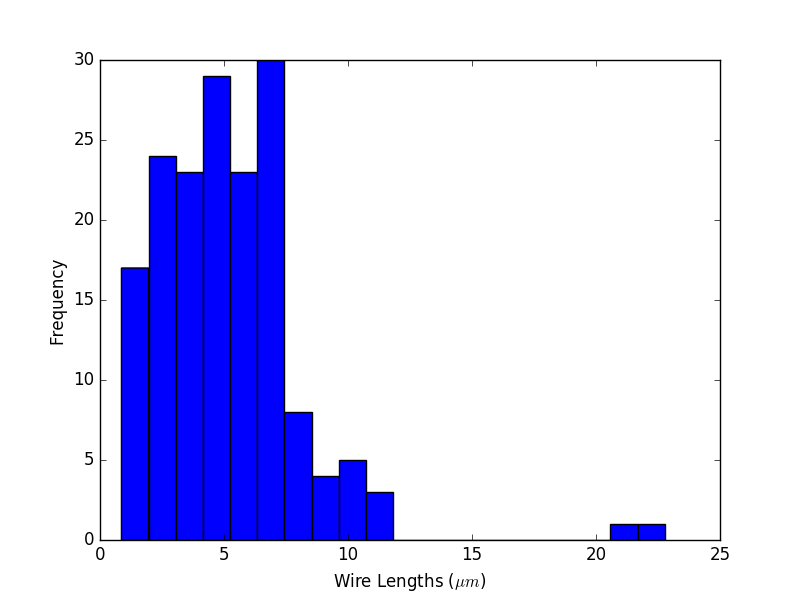
\includegraphics[width=0.7 \columnwidth]{Images/Chapter3/wireLengthDist.png}
\caption{\fontsize{12pt}{11pt}\selectfont Frequency distribution of the wire lengths obtained the digitised NWN shown in Fig. \ref{fig: digitisedNWNs} b). There are a large number of short NWNs with a peak in frequency at around $7 \mu m$ and a quick drop off in wire lengths after this. The mean wire length for this sample is $5.16 \mu m$ and median wire length $4.89 \mu m$.}%
\label{fig: wireLength_Dist}
\end{figure}


\begin{comment
\begin{table}
\begin{center}
\begin{tabular}{| c | c c c c c c c c |}
\hline
network & $n_w$ & $R_s^{EXP}$ & $R_0$  & $\Delta$ & $a$ & $\Delta/a = R_j^{MNR}$ & $R_s^{EXP}/a = R_j^{JDA}$
 & $\gamma$ \\ 
\hline
1 & 0.28 & 84.42 & 46.43 & 37.99 & 1.37 & 27.73 & 61.62 & 0.45 \\ 
2 & 0.16 & 159.95 & 92.05 & 67.9 & 2.47 & 27.52 & 64.83 & 0.42 \\ 
3 & 0.16 & 177.14 & 60.99 & 116.15 & 1.93 & 60.07 & 91.61 & 0.65 \\ 
4 & 0.49 & 18.8 & 12.86 & 5.94 & 0.44 & 13.38 & 42.35 & 0.31 \\ 
5 & 0.64 & 23.77 & 12.09 & 11.67 & 0.27 & 43.39 & 88.38 & 0.49 \\ 
6 & 0.35 & 180.5 & 32.91 & 147.58 & 0.97 & 152 & 185.91 & 0.82 \\ 
7 & 0.63 & 14.85 & 8.9 & 5.94 & 0.17 & 35.03 & 87.58 & 0.4 \\ 
8 & 0.47 & 29.89 & 9.3 & 11.58 & 0.22 & 52.52 & 135.56 & 0.55 \\ 
9 & 0.17 & 56.2 & 37.9 & 18.28 & 1.20 & 15.28 & 46.98 & 0.32 \\ 
10 & 0.39 & 67.27 & 32.85 & 34.42 & 1.01 & 33.96 & 66.37 & 0.51 \\ 
11 & 0.2 & 233.15 & 71.42 & 161.72 & 2.31 & 69.89 & 100.76 & 0.69 \\ 
12 & 0.57 & 51.06 & 20.93 & 30.13 & 0.59 & 51.01 & 86.44 & 0.59 \\ 
13 & 0.17 & 220.54 & 52.14 & 168.4 & 1.34 & 125.88 & 164.85 & 0.76 \\ 
14 & 0.37 & 33.98 & 22.03 & 11.95 & 0.53 & 22.71 & 64.58 & 0.35 \\ 
15 & 0.14 & 194.33 & 77.15 & 117.18 & 1.90 & 61.57 & 102.11 & 0.6 \\ 
16 & 0.26 & 54.54 & 26.39 & 28.14 & 0.73 & 38.33 & 74.29 & 0.51 \\ 
17 & 0.24 & 50.38 & 28.18 & 22.2 & 0.83 & 26.6 & 60.37 & 0.44 \\ 
18 & 0.12 & 109.12 & 42.7 & 66.42 & 0.98 & 67.47 & 110.85 & 0.61 \\ 
19 & 0.21 & 61.88 & 58.68 & 3.19 & 1.40 & 2.28 & 44.23 & 0.05 \\ 
20 & 0.29 & 42.15 & 20.78 & 21.36 & 0.56 & 38.28 & 75.54 & 0.51 \\ 
21 & 0.28 & 54.17 & 35.44 & 18.73 & 0.80 & 23.33 & 67.47 & 0.34 \\ 
22 & 0.14 & 103.62 & 70.48 & 33.14 & 2.10 & 15.76 & 49.28 & 0.32 \\ 
23 & 0.35 & 34.65 & 21.97 & 12.68 & 0.42 & 29.92 & 81.76 & 0.36 \\ 
24 & 0.29 & 41.49 & 19.19 & 22.3 & 0.51 & 43.68 & 81.27 & 0.54 \\ 
25 & 0.37 & 58.31 & 19.81 & 38.5 & 0.68 & 56.78 & 86.00 & 0.66 \\ 
26 & 0.36 & 42.93 & 17.68 & 25.24 & 0.48 & 53.03 & 90.20 & 0.59 \\ 
27 & 0.43 & 39.33 & 16.23 & 23.1 & 0.48 & 48.18 & 82.03 & 0.59 \\ 
28 & 0.35 & 56.12 & 32.02 & 24.1 & 1.10 & 21.92 & 51.04 & 0.43 \\ 
29 & 0.19 & 188.04 & 66.52 & 121.52 & 2.35 & 51.75 & 80.08 & 0.65 \\ 
30 & 0.22 & 76.68 & 38.04 & 38.64 & 1.00 & 38.54 & 76.48 & 0.5 \\ 
\hline
\end{tabular}
\caption{\fontsize{12pt}{11pt}\selectfont Wire densities (n), characteristic junction resistances ($Delta$/a) of all Ag NWN samples
obtained by fitting the measured sheet resistance ($R_s^{exp}$) with the calculated curves $R_s$ vs. $R_j$ derived
within MNR. Values of $\Delta$, $R_0$ as well as the optimization-capacity coefficient ($\gamma$) are also depicted. PUT IN APPENDIX}
\label{fig:table}
\end{center}
\end{table}
\end{comment}
